\section{Quality drivers embedded in URDAD}


\begin{frame}{Semantic quality}

  Model quality impacted by quality of modeling language.
      \begin{itemize}
	\item Define semantics via metamodel or ontology.
      \end{itemize}
    \pause
    \begin{block}{Qualities of modeling language:}
      \begin{itemize}
	\item<+-| alert@+> {\em Completeness}
	\begin{itemize}
	  \item Formal lang: power to express statements needed for URDAD.
	    \begin{itemize}
	      \item All meaning to be conveyed can be conveyed.
	    \end{itemize}
	  \item Informally verified through
	    \begin{itemize}
	      \item Analyze URDAD process \& models for required semantics.
	      \item Empirically tested via example models.
	    \end{itemize}
	\end{itemize}
	\item<+-| alert@+> {\em Consistency}
	  \begin{itemize}
	    \item Metamodel/ontology is instantiable
	    \item Verified: transform to ontology \& assessed consistency using logical reasoner.
	  \end{itemize}
	\item<+-| alert@+> {\em Complexity}
	  \begin{itemize}
	    \item Assessed by counting classes, relationships \& constraints.
	    \item Much lower than for UML (generic language).
			 \begin{itemize}
				\item UML: 16x more classes, 7x more relationships.
			 \end{itemize}
	  \end{itemize}
      \end{itemize}
    \end{block}
\end{frame}

%--------------------------------------------------%

\begin{frame}{Example: Language elements for contract specification}

  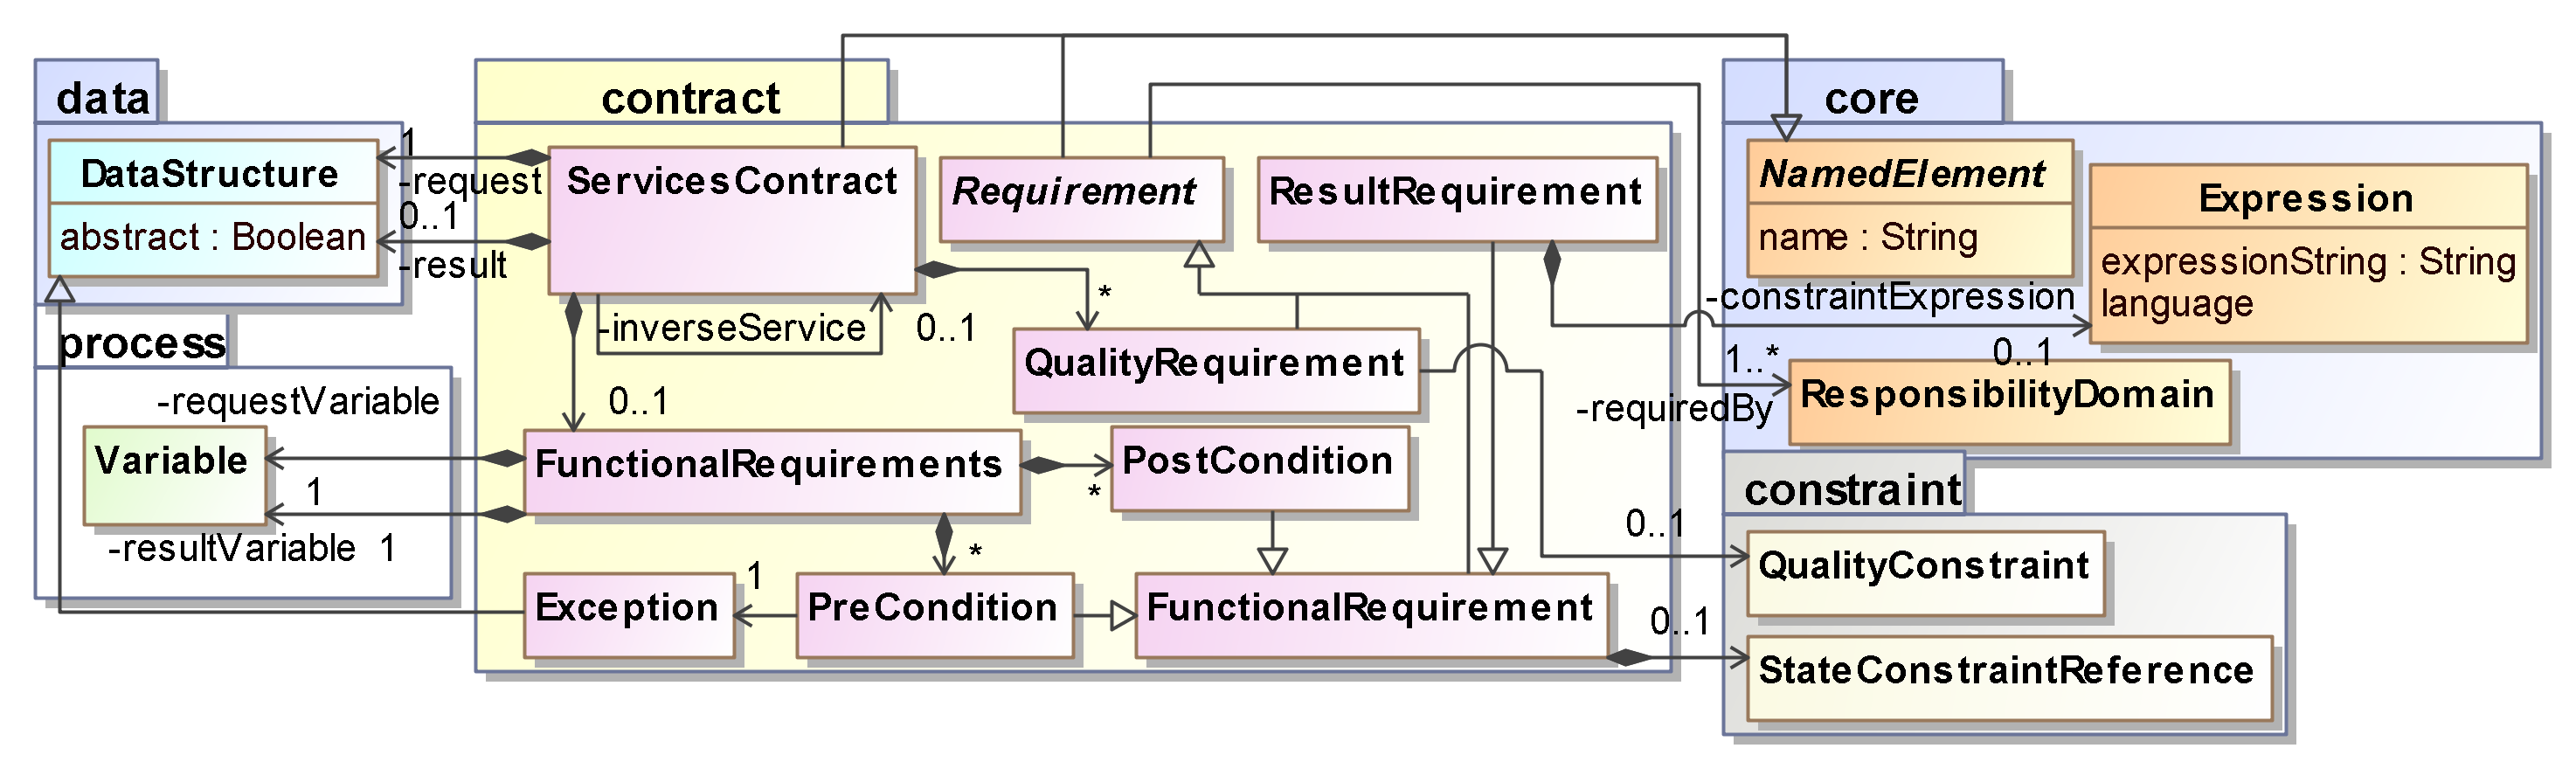
\includegraphics[width=100mm]{contract}

\end{frame}


%----------------------------------------------------------------%

\begin{frame}{Syntactic quality}
   Ensure statements made in model comply to syntax rules of metamodel.
		\begin{itemize} 
			 \item Important for model validation, code, test \& documentation generation
		  \end{itemize}
  \pause
  \begin{block}{Syntactic quality drivers}
    \begin{itemize}
		  \item<+-| alert@+> Define concrete syntax for encoding of models.
			 \begin{itemize}
				\item Text-based or diagrammatic.
				\item Bi-directional mapping between syntax \& metamodel.
				\item Enforces URDAD semantics \& model structure.
			 \end{itemize}
		  \item<+-| alert@+> Generate validating editor for concrete syntax.
			 \begin{itemize}
				\item Done using MDA tool suite.
			 \end{itemize}
		  \item<+-| alert@+> Use model validators
			 \begin{itemize}
				\item Compliance to metamodel structure.
				\item Adherance to metamodel constraints.
			 \end{itemize}
    \end{itemize}
  \end{block}

\end{frame}

%----------------------------------------------------------------%

\begin{frame}[fragile]
\frametitle{Example: Service contract specification (1/2)}

\lstset{language=urdad,label=contractTextSyntax}
\begin{lstlisting}[numbers=left,escapechar=|]
ServiceContract enrollForPresentation
{
 FunctionalRequirements receiving Variable enrollForPresentationRequest ofType EnrollForPresentationRequest
 {
  PreCondition enrollmentPrerequisitesMet requiredBy (TrainingRegulator Student) raises EnrollmentPrerequisitesNotSatisfiedException checks constraint enrollmentPrerequisitesForPresentationMet with ValueOf enrollForPresentationRequest
  PostCondition enrollmentProcessPerformed requiredBy (Student Client TrainingRegulator) ensures constraint studentEnrolledForPresentation          with ValueOf studentEnrolledRequest constructedUsing doSequential
  {
   create Variable studentEnrolledRequest ofType StudentEnrolledRequest
   set Query OCL:"studentEnrolledRequest.personIdentifier" equalTo Query OCL:"enrollForPresentationRequest.personIdentifier"                            
   set Query OCL:"studentEnrolledRequest.presentationIdentifier" equalTo Query OCL:"enrollForPresentationRequest.presentationIdentifier"                            
  }  

\end{lstlisting}
\end{frame}

\begin{frame}[fragile]
\frametitle{Example: Service contract specification (2/2)}
          
\lstset{language=urdad,label=contractTextSyntax2}
\begin{lstlisting}[numbers=left,escapechar=|]
  ...
  PostCondition invoiceIssued ...
 }            
 Request DataStructure EnrollForPresentationRequest 
 {
  has identification presentationIdentifier identifying Presentation
  has identification studentIdentifier identifying Person
  has identification clientIdentifier identifying LegalEntity         
 }
 Result DataStructure EnrollForPresentationResult { ... } 
}
\end{lstlisting}
\end{frame}

%---------------------------------------------------------------%

\begin{frame}{Simplicity}
  Inverse measure of complexity.
		\begin{itemize} 
			 \item Important because reduces cost, risk \& improves maintainability.
		  \end{itemize}
  \pause
  \begin{block}{Simplicity drivers}
	 \begin{itemize}
		\item<+-| alert@+> Use DSL to provide compact, precise language.
		  \begin{itemize}
			 \item Reduce model size \& improves understandability.
		  \end{itemize}
		\item<+-| alert@+> Ensure all process activities address functional requirements.
		  \begin{itemize}
			 \item Enforced through metamodel.
		  \end{itemize}
		\item<+-| alert@+> Enforce single responsibility principle
			 \begin{itemize}
				\item Assignment of services to responsibility domains.
			 \end{itemize}
	 \item<+-| alert@+> No duplication of statements
		  \begin{itemize}
			 \item Only one way to specify things.
		  \end{itemize}
	 \end{itemize}
  \end{block}
\end{frame}

%---------------------------------------------------------------%

\begin{frame}{Model completeness}
	 The extend to which the model has all elements required for the model use cases
		\begin{itemize} 
			 \item e.g.\ code, test \& documentation generation.
		  \end{itemize}
  \pause
  \begin{block}{Model completeness drivers}
	 \begin{itemize}
		\item<+-| alert@+> Structural completeness criteria
		  \begin{itemize}
			 \item Certain minimal structure enforced through metamodel.
		  \end{itemize}
		\item<+-| alert@+> Process completeness
		  \begin{itemize}
			 \item All functional requirements addressed.
		    \item Enforced through metaodel constraint.
		  \end{itemize}
		\item<+-| alert@+> No enforced completeness on levels of granularity.
		  \begin{itemize}
			 \item Decoupled via services contracts.
			 \item Service provider need not be designed - could be plugged in.
		  \end{itemize}
		\item<+-| alert@+> Process assistance for completeness via process steps with
		  \begin{itemize}
			 \item defined inputs \& outputs, and
			 \item defined process tasks.
		  \end{itemize}
	 \end{itemize}
  \end{block}
\end{frame}

%---------------------------------------------------------------%

\begin{frame}{Model Consistency}
  Consistency often problematic in UML models
    \begin{itemize}
     \item Different UML models structurally and even semantically very different.
     \item Consistency issues across diagrams (e.g. sequence, activity diagrams \& state charts).
    \end{itemize}
  \pause
  \begin{block}{Model consistency drivers}
    \begin{itemize}
      \item<+-| alert@+> Repeatable process with defined inputs, outputs \& tasks for each process step.
      \item<+-| alert@+> Enforced model structure \& semantics through metamodel.
		  \begin{itemize}
			\item Does not allow duplicate specifications
		  \end{itemize}
    \end{itemize}
  \end{block}
\end{frame}

%---------------------------------------------------------------%

\begin{frame}{Model Cohesion}
  Cohesion refers the extend to which structural realtionships map onto conceptual and functional relationships.
    \begin{itemize}
     \item Important for localized maintenance, easy finding of model elements, testability reusability and understandability.
     \item High model cohesion results in code with high cohesion.
    \end{itemize}
  \pause
  \begin{block}{Model cohesion drivers}
	 \begin{itemize}
	 \item<+-| alert@+> Responsibility localization
		  \begin{itemize}
			 \item Contracts contain only services from same responsibility domain.
			 \item ``Encouraged'' by process.
		  \end{itemize}
	 \item<+-| alert@+> Services as cohesive, self-contained units
		  \begin{itemize}
			 \item Statelessness enforced by metamodel.
			 \item Each service must address complete functional requirement at some level of granularity.
		  \end{itemize}
	 \end{itemize}
  \end{block}
\end{frame}

%---------------------------------------------------------------%

\begin{frame}{Traceability}
  Traceability refers to the ability to trace rationale, satisfaction, dependency and evolution.
    \begin{itemize}
     \item Important for estimation, design validation and maintenance.
     \item Validation for both, sufficiency and necessity.
    \end{itemize}
  \pause
  \begin{block}{Traceability drivers}
    \begin{itemize}
		\item<+-| alert@+> Include satisfaction, dependency and rationale links in model.
		\item<+-| alert@+> Rationale links
		  \begin{itemize}
		   \item  only indirectly through link of process activity to functional requirement \& functional requirement to stakeholder.
		  \end{itemize}
      \item<+-| alert@+> Satisfaction links
		  \begin{itemize}
			 \item between services and service contracts.
		  \end{itemize}
      \item<+-| alert@+> Dependency links throughout.
		  \begin{itemize}
			 \item e.g. dependencies between services across levels of granularity.
		  \end{itemize}
		\item<+-| alert@+> Evolutionary links through version control.
    \end{itemize}
  \end{block}
\end{frame}

%----------------------------------------------------------------%

\begin{frame}[fragile]
\frametitle{Example: Service specification (1/2)}

\lstset{language=urdad,label=serviceTextSyntax}
\begin{lstlisting}[numbers=left,escapechar=|]
Service enrollForPresentationImpl realizes enrollForPresentation receiving Variable enrollForPresentationRequest ofType EnrollForPresentationRequest
{
 use checkStudentSatisfiesEnrollmentPrerequisites toAddress (enrollmentPrerequisitesMet)
 use issueInvoice toAddress (financialPrerequisitesSatisfied invoiceIssued) 
 ...
 Process doSequential
 {
  create Variable checkStudentSatisfiesEnrollmentPrerequisitesRequest ofType CheckStudentSatisfiesEnrollmentPrerequisitesRequest               
  set Query OCL:"enrollForPresentationRequest.studentIdentifier" equalTo Query OCL:"checkEnrollmentPrerequisitesRequest.studentIdentifier"
  set Query OCL:"enrollForPresentationRequest.presentationIdentifier" equalTo Query OCL:"checkEnrollmentPrerequisitesRequest.presentationIdentifier"
  ...
\end{lstlisting}
\end{frame}
                   

\begin{frame}[fragile]
\frametitle{Example: Service specification (2/2)}
\lstset{language=urdad,label=serviceTextSyntax2}
\begin{lstlisting}[numbers=left,escapechar=|]
  requestService checkStudentSatisfiesEnrollmentPrerequisites with checkStudentSatisfiesEnrollmentPrerequisitesRequest yielding Variable checkStudentSatisfiesEnrollmentPrerequisitesResult ofType CheckStudentSatisfiesEnrollmentPrerequisitesResult
  choice
  {
   if Constraint enrollmentMeetsPrerequisitesMet OCL:"checkStudentSatisfiesEnrollmentPrerequisitesResult.enrollmentPrerequisitesMet = true" doSequential
   {
    ...
    requestService issueInvoice with issueInvoiceRequest yielding Variable issueInvoiceResult ofType IssueInvoiceResult
    {
     on FinancialPrerequisitesNotSatisfiedException raiseException FinancialPrerequisitesNotSatisfiedException
    }
    ...
    returnResult  enrollForPresentationResult
   }
   else raiseException EnrollmentPrerequisitesNotSatisfiedException
  }
 }
}                 
\end{lstlisting}
\end{frame}

%---------------------------------------------------------------%

\begin{frame}{Model modifiability}
  Modifiability refers to the ease with which the model can be modified.
    \begin{itemize}
     \item Important for maintenance in context of change requests and refactorization.
    \end{itemize}
  \pause
  \begin{block}{Modifiability drivers}
	 \begin{itemize}
	   \item<+-| alert@+> Decoupling via services contracts
		  \begin{itemize}
			 \item Modifiability through decoupling.
			 \item ``Enforced'' by process \& metamodel.
		  \end{itemize}
	   \item<+-| alert@+> Defined levels of granularity
		  \begin{itemize}
			 \item Process includes step to check whether additional levels of granularity should be defined.
			 \item Requirements engineer verifies whether any services at any level of granularity can be combined into single, cohesive, higher-level service.
		  \end{itemize}
		\item<+-| alert@+> Simplicity and hence its quality drivers also improve modifiability.
	 \end{itemize}
  \end{block}
\end{frame}

%---------------------------------------------------------------%

\begin{frame}{Reusability}
  Reusability refers to the ease with which model elements can be reused.
    \begin{itemize}
     \item Important for reducing development \& maintenance cost \& risk, as well as consistency.
    \end{itemize}
  \pause
  \begin{block}{Reusability drivers}
	 \begin{itemize}
	 \item<+-| alert@+> All services realize services contracts
		  \begin{itemize}
			 \item Modifiability through decoupling.
			 \item ``Enforced'' by process \& metamodel.
		  \end{itemize}
		\item<+-| alert@+> Optimize levels of granularity
		\item<+-| alert@+> Stateless, self-contained services.
		\item<+-| alert@+> Cohesion and hence its quality drivers.
		\item<+-| alert@+> Linkage btw service \$ contract aids service provider discoverability.
		\item<+-| alert@+> Enforced adapter layer.
	 \end{itemize}
  \end{block}
\end{frame}
%---------------------------------------------------------------%

\begin{frame}{Testability}
  Testability refers to the ease with which the model or its implementation mapping can be tested.
    \begin{itemize}
     \item Important for model \& code validation.
    \end{itemize}
  \pause
  \begin{block}{Teatability drivers}
	 \begin{itemize}
		\item<+-| alert@+> Fully specified services contracts
		  \begin{itemize}
			 \item In service-oriented paradigm, services can only be tested by
				\begin{itemize}
				  \item Extracting information about environment using other services.
				  \item Assessing constraints on obtained information.
				\end{itemize}
		  \end{itemize}
		\item<+-| alert@+> Metamodel
		  \begin{itemize}
			 \item Contract has constraint as either pre- or post-condition.
			 \item Same state constraint can be pre- and post- condition for different services.
		  \end{itemize}
	 \end{itemize}
  \end{block}
\end{frame}

%----------------------------------------------------------------%

\begin{frame}[fragile]
\frametitle{Example: State constraint specification}

\lstset{language=urdad,label=serviceTextSyntax}
\begin{lstlisting}[numbers=left,escapechar=|]
StateConstraint studentEnrolledForPresentation receiving Variable enrollForPresentationRequest ofType EnrollForPresentationRequest
{
 stateAssessmentProcess doSequential
 {
  create Variable getEnrollmentsRequest ofType GetEnrollmentsRequest
  set Query OCL:"getEnrollmentsRequest.presentationIdentifier" equalTo Query OCL:"enrollForPresentationRequest.presentationIdentifier"
  requestService getEnrollments with getEnrollmentsRequest yielding Variable getEnrollmentsResult ofType GetEnrollmentsResult
 }
 Constraint OCL:"getEnrollmentsResult.enrollments.includes (enrollForPresentationRequest.personIdentifier)"
}
\end{lstlisting}
\end{frame}

\begin{frame}[fragile]
  \frametitle{Summary of quality drivers in URDAD}

\begin{scriptsize}
\begin{tabular}{|l|cc|cccccccc|} \hline
\multirow{4}{*}{\bf Quality-driver} & \multicolumn{10}{c|}{\bf Model qualities} \\ \cline{2-11}
& & & \multicolumn{8}{c|}{Pragmatic model qualities}\\ \cline{4-11}
    & \begin{sideways}Semantic\end{sideways} & \begin{sideways}Syntactic\end{sideways}  & \begin{sideways}Simplicity\end{sideways}
    & \begin{sideways}Completeness\end{sideways} & \begin{sideways}Modifiability\end{sideways} & \begin{sideways}Consistency\end{sideways}
    & \begin{sideways}Decoupling\end{sideways} & \begin{sideways}Cohesion\end{sideways} & \begin{sideways}Reusability\end{sideways}
    & \begin{sideways}Traceability\end{sideways} \\ \hline
%                                       Semantic     Syntax        Simplicity  Completeness   Modifiable  Consistent  Decoupled    Cohesion     Reuse        Traceable
Define metamodel or ontology                   & \checkmark & \checkmark & \checkmark & \checkmark & \checkmark & \checkmark & \checkmark &            &            & \checkmark \\
Define concrete DSL grammars                   &            & \checkmark & \checkmark &            & \checkmark &            &            &            &
& \\
Define levels of granularity                        &            &            & \checkmark &            & \checkmark &            &            &            &
\checkmark & \checkmark \\
Decouple services via contracts                &            &            & \checkmark &            & \checkmark &            & \checkmark &            & \checkmark & \checkmark \\
Single reponsibility principle           &            &            & \checkmark &            & \checkmark &            &            & \checkmark & \checkmark & \checkmark \\
Testable pre- \& post-conditions       &            &            &            & \checkmark & \checkmark & \checkmark &            &            &            &  \\
Localize controll logic             &            &            & \checkmark &            & \checkmark &            & \checkmark & \checkmark & \checkmark & \checkmark \\
Include traceability links                     &            &            & \checkmark & \checkmark & \checkmark & \checkmark &            &            &            & \checkmark \\ \hline
\end{tabular}
\end{scriptsize}

\end{frame}
